\section{Dodatkowe narzędzia}

Poza głównym silnikiem symulacyjnym projekt oferuje kilka dodatkowych narzędzi, a jednym z nich jest moduł uproszczonego interfejsu graficznego użytkownika. Interfejs jest podzielony na dwie części --- podgląd przebiegu rozgrywki między dwoma agentami sterowanymi przez funkcje oceny oraz prosty kreator talii \cite{sabberstone_gui_wiki}. Mimo ograniczonej funkcjonalności jest to użyteczne narzędzie diagnostyczne i demonstracyjne. Wygląd interfejsu przedstawiono na rysunku~\ref{fig:sabberstone_gui}. Moduł został jednak oznaczony jako przestarzały i zastąpiony klientem opartym na silniku Unity3D --- nowy interfejs oferuje wizualizację rozgrywki w czasie rzeczywistym poprzez komunikację z serwerem gry \cite{sabberstone_github}.

\begin{figure}[!ht]
    \centering
    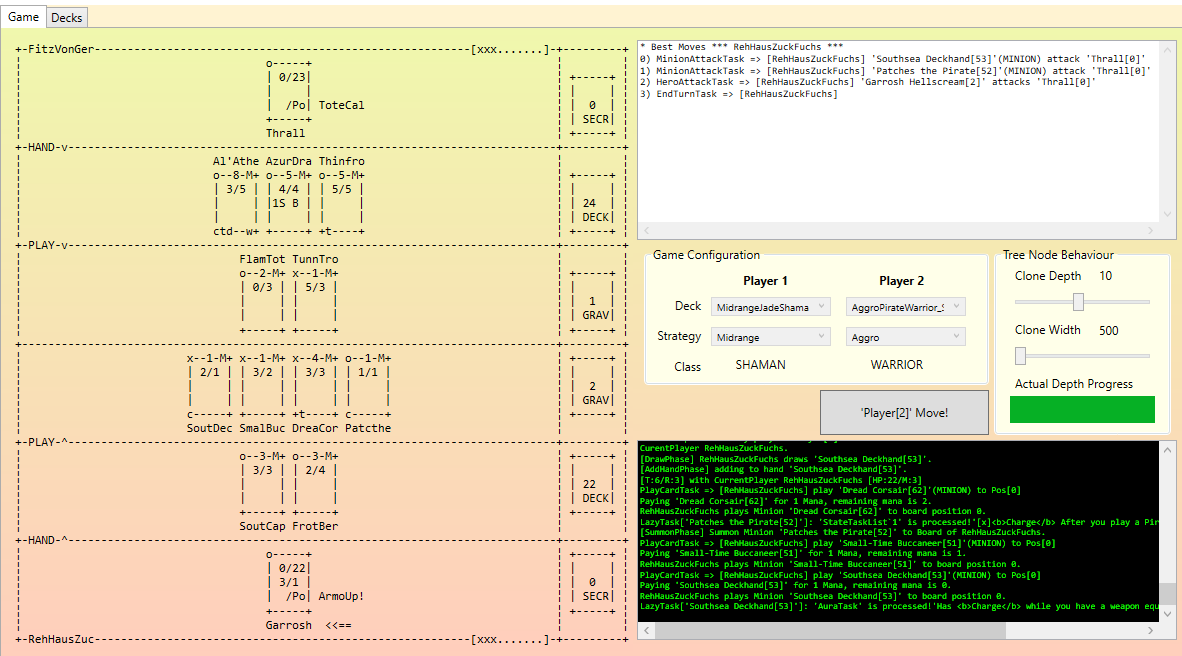
\includegraphics[width=0.95\textwidth]{images/simpleui.PNG}
    \caption{Interfejs graficzny \texttt{SabberStoneGui} --- widok rozgrywki w reprezentacji tekstowej (lewa strona) z aktualnym stanem planszy obu graczy oraz panel konfiguracji (prawa strona) umożliwiający wybór talii, strategii i parametrów przeszukiwania. Źródło:~\cite{sabberstone_gui_wiki}.}
    \label{fig:sabberstone_gui}
\end{figure}

Kolejnym rozszerzeniem projektu jest architektura klient-serwer oparta na protokole gRPC --- moduł ten umożliwia implementację agentów w dowolnym języku programowania, a nie tylko w C\# \cite{sabberstone_github}. Oznacza to możliwość bezpośredniego zastosowania bibliotek uczenia maszynowego dostępnych np. w ekosystemie Pythona, takich jak PyTorch czy TensorFlow, bez konieczności przepisywania kodu do C\#. Silnik działa wówczas jako autonomiczny serwer, a komunikacja z agentami odbywa się przez sieć lokalną lub zdalną, co ilustruje rysunek~\ref{fig:sabberstone_unity}.

\begin{figure}[ht]
    \centering
    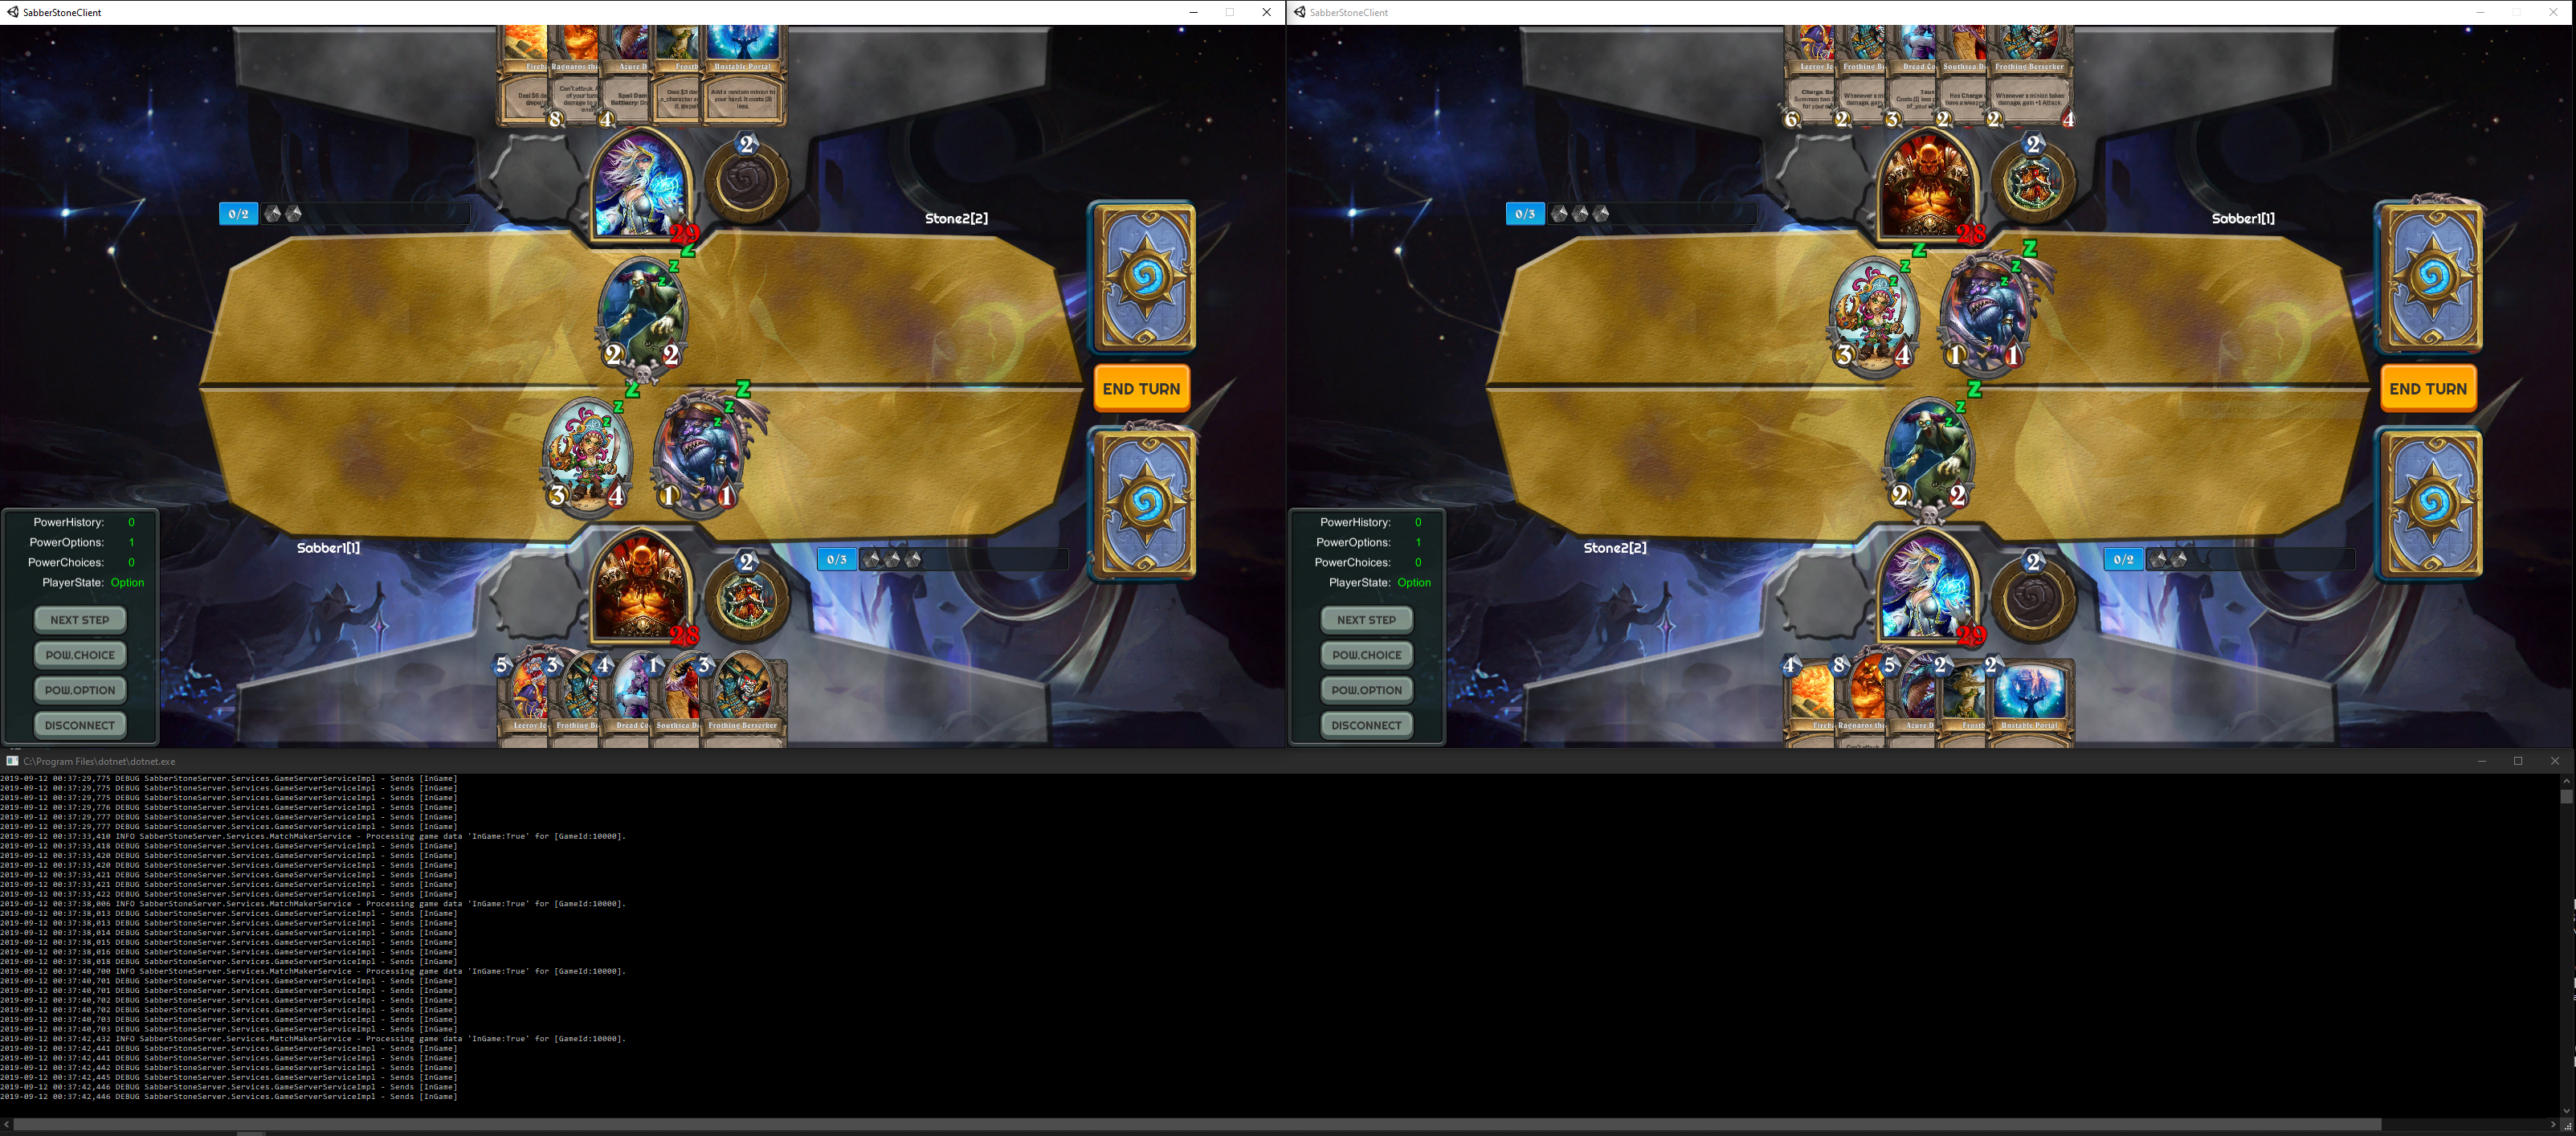
\includegraphics[width=0.95\textwidth]{images/clientserver.png}
    \caption{Klient Unity3D (\texttt{SabberStoneUnityClient}) wizualizujący rozgrywkę w czasie rzeczywistym. Widoczne są dwa równoległe okna klientów komunikujących się z serwerem SabberStone przez protokół gRPC, wraz z logiem serwera w dolnej części ekranu. Źródło:~\cite{sabberstone_github}.}
    \label{fig:sabberstone_unity}
\end{figure}
